\documentclass{article}
\usepackage{times}
\usepackage{ijcai16}
\usepackage{times}
\usepackage{graphicx}
\usepackage{amsmath}
\usepackage{amsthm, amssymb}
\usepackage{enumerate}
\usepackage{fullpage}
\usepackage{hyperref}
\usepackage{soul}
\usepackage{xcolor}
\usepackage{float}
\usepackage{comment}
\restylefloat{table}
\usepackage{listings}
\usepackage{color} %red, green, blue, yellow, cyan, magenta, black, white
\definecolor{mygreen}{RGB}{28,172,0} % color values Red, Green, Blue
\definecolor{mylilas}{RGB}{170,55,241}
\usepackage{fancybox}
\usepackage{framed}
\usepackage{mathrsfs}
\usepackage{url}
\usepackage{paralist}

\hypersetup{breaklinks=true}
\urlstyle{same}


\graphicspath{{Pictures/}}

\begin{document}
\title{Data Mining Corporate Emails to Model Employee Behaviors and Analyze Organizational Structure}
%\title{Organizational Relationship Classification From Data Mining Corporate Email Metadata}
\author{Kayla Straub\\
        Virginia Tech, Blacksburg, Virginia\\
        kstraub@vt.edu}
\maketitle

\begin{abstract}
Email correspondence has become the predominant method of communication for businesses.  If not for the inherent privacy concerns, this electronically searchable data could be used to better understand how employees interact. For example, after the Enron dataset was made available, researchers were able to provide great insight into employee behaviors based on the available data despite the many challenges with that dataset.  The work in this paper demonstrates the application of a suite of methods to an appropriately anonymized email dataset created from volunteers' email metadata.  This new dataset, from an internal email server, is first used to validate machine learning and feature extraction algorithms and then to generate insight into the interactions within the center.  Based solely on email data, a random forest  modeled behavior patterns and accurately classified not only participants in the study but also other members of the center who were connected to participants through email.  Furthermore, the data revealed relationships not present in the formal operating structure.  The result is a much fuller understanding of the center's internal structure than can be found in the official organization chart.
\end{abstract}

\section{Introduction}
Talk about applications of determining work structure from email behavior? \\
Why problem is important/hard/unsolved\\

Organization charts do not always accurately reflect relationships within workplace.  This paper seeks to determine if true behaviors are instead exhibited in corporate email communication patterns.

Email is a pervasive medium for communication in modern society - particularly in the workplace.  In 2015, there were estimated over 2.6 billion email users, and it is projected that by the end of 2019, over one third of the global population will be using email.  In fact, the average business email user sends or receives 112 emails per day.  Corporate email alone accounts for 54.7\% of worldwide email traffic \cite{radicati_emails_2015}. Retention of large email archives has become common practice with decreasing memory size and cost \cite{fisher_revisiting_2006}.  In that study, out of 600 employees at a high-tech company, the average employee had 28,660 emails stored in 133 folders which is a significant increase from 10 years earlier.  This trove of interesting information can be leveraged to analyze the relationships between coworkers.
\par
The following section summarizes related works in this area.  Section \ref{Data Collection} describes the process of data collection and some statistics of the dataset.  The features extracted from the data are described in Section \ref{Features}, and the analyses using these features are covered in Section \ref{Analysis}.  The results of the analysis are presented in Section \ref{Results}.  Section \ref{Conclusions} concludes the paper and presents opportunites for future work.  

\section{Related Works} \label{Related Works}
Email has been a common research topic over the past decade.  This is in part because  the Enron email dataset was released in 2004 \cite{klimt_introducing_2004}, allowing researchers access to a rich collection of real-world corporate emails.  This dataset has been extensively researched on topics including spam classification \cite{martin_analyzing_2005}, \cite{gaber_e-mail_2016}, \cite{shams_classifying_2013}; email categorization \cite{he_novel_2014}, \cite{keila_structure_2005}; and recipient prediction \cite{sofershtein_predicting_2015}, \cite{hu_towards_2012}.  However, there are known flaws and discrepancies with even the most recent versions of this dataset -- ranging from misspelled email addresses \cite{nordbo_data_2014} to duplicate emails \cite{waterman_big_2014}. In one of the most popular forms of the dataset, \cite{shetty_enron_2004}, the database includes 253,735 emails sent as ``CC'' and  253,713 emails sent as ``BCC''.  Further inspection reveals that emails sent as one type or the other were almost always mistakenly recorded as both.
\par
The existing literature on analyzing social email behavior is mainly divided into two categories: feature-based and social-based \cite{tang_email_2013}.  Feature-based methods calculate statistics based only on email patterns while social-based methods extract information from representing the email traffic as a social graph.
\par
Using features extracted from email metadata, \cite{yelupula_social_2008} was able to cluster levels of management at Enron. In addition to email traffic statistics, using features such as the presence of different email attachment types and the length of emails were shown to successfully categorize email behavior in \cite{martin_analyzing_2005}.
\par
Relational ties can be modeled as a graph network where nodes represent people and edges represent interactions.  This is a useful model because many statistics can be calculated from the layout of a social graph \cite{wasserman_social_1994}.  A common metric that has been shown to indicate importance in a social graph is betweenness centrality, which comes in several different flavors, and was first developed by \cite{freeman_set_1977}.  Betweenness centrality is a measure of how many shortest paths in a graph travel over each node.  A node with high betweenness centrality in a social graph has been shown to represent a high degree of influence on other nodes.  As \cite{tyler_email_2003} shows, a betweenness centrality algorithm can be used on a social graph to determine community structures within an organization.  However, other metrics have been used successfully as well.  For example, \cite{wilson_discovery_2009} detected the most important email users within a corporate network without using betweenness as a feature.  Instead, they used: degree, the number of edges connected to a node; density, the ratio of actual edges to the number of possible edges; and proximity prestige, the ratio of nodes that can reach a node $i$ to the average distance from those nodes to $i$.
\par
Some research has been done in trying to combine the two different types of features.  An example of this approach is seen in \cite{rowe_automated_2007}, which combined features such as number of emails, response time, cliques, and degree centrality into a ``Social Score'' which was used to rank Enron employees.  The purpose of this paper is to further unite the two branches of research by aggregating old and novel email traffic statistics with social graph features and applying them to a new, clean dataset.

\section{Data Collection} \label{Data Collection}
Over the past decade, the Enron dataset has been widely used to study email behaviors because it is one of the only datasets available comprised of real-world corporate emails.  A list of ground truth job titles was compiled by \cite{shetty_status_2004}.  However, there are issues with these labels.  For example, Jeff Dasovich had the most emails out of any employee in the database, and is labeled as "employee".  In reality, Jeff Dasovich served as the Director for State Government Affairs. Additionally, over the period that the dataset covers, Enron was undergoing turmoil where directors changed and job titles shifted.  Instead of working with uncertain labels, we decided to generate a new dataset from an organization with which we had intimate knowledge, our own center.  
\par
The center divides its employees into six main areas: directors, graduate students, operations, outreach, project management, and research.  These labels are very stable.  Furthermore, we understand the intimate details for the rare case where the label has changed, i.e. when a graduate student graduates and gets hired on as a researcher. We also have inside knowledge as to personal relationships within the center which may be revealed in the data.
\par 
An Internal Review Board approved the study after reviewing a thorough proposal.  Each of the 37 participants signed a waiver that detailed the specifics of the study.   The following information was extracted from participants' emails:  
\begin{compactitem}
\item Destination and source email address
\item Email time stamp
\item Subject prefix (if any)
\item Hash of subject after removing prefix
\item Hash of body text
\item Length of subject in characters
\item Length of body text in characters
\item Whether email was encrypted/signed
\end{compactitem}
Table \ref{tab:db_stats} compares statistics between our dataset and the Enron corpus.  Note that our emails involve less people over a longer period of time.  
Special care was taken to protect the privacy of those involved in the study.  During the collection process, all subject and body text was hashed, and all email  metadata was stored in a database using scripts without any researchers observing any email details. Furthermore, any identifying information has been omitted from this report.
\par
In an effort to increase the number of employees to analyze, statistics were also calculated for former center employees or others who had known affiliation with the center.  These second-ring employees were included in the study if their job title was known and if they were involved in at least 100 emails in the database.  This added 32 subjects to the study, for a total of 69 employees to analyze.

\begin{table}[H]
\centering
\caption{Comparing our database to the Enron email corpus.  Our internal database is more modern, has more emails, and covers a longer time period.  However, it is comprised of less people than the Enron dataset.}
\label{tab:db_stats}
\begin{tabular}{l|l|l|ll}
\cline{2-3}
                                               & Our Database    & Enron         &  &  \\ \cline{1-3}
\multicolumn{1}{|l|}{Time Period}              & 11/2012-11/2015 & 1/2000-9/2002 &  &  \\
\multicolumn{1}{|l|}{Distinct Addresses} & 32,118          & 75,406        &  &  \\
\multicolumn{1}{|l|}{Participants}             & 32              & 149           &  &  \\
\multicolumn{1}{|l|}{Distinct Emails}          & 585,096         & 252,759       &  &  \\ \cline{1-3}
\end{tabular}
\end{table}

\section{Features} \label{Features}
In total, 101 different features were extracted from the email data: 70 traffic-based and 31 graph-based.  Below, all features will be described in both categories.  This ranking comes from an information gain ranker which was used to determine the most important features.  Section 5 goes into more detail on this topic.

\subsection{Traffic-Based Features}
The traffic-based features were those extracted purely from email metadata.  Some of these features were very basic, such as total number of emails, total sent, and total received.  Other features came from the types of emails.  For example, the number of emails sent and received were counted for each of the recipient types: to, cc, and bcc.  Similarly, the number of emails sent and received as replies or forwards were also used as features.  The number of unique email addresses communicated with and the number of unique email subjects involving each person, both sent and received, were counted as features to be used.  The average number of recipients on emails sent and received for each participant were calculated.  It was hypothesized that staff members had more inter-center communications while graduate students communicated more with the university.  To investigate this, the number of emails sent and received from within the center and within the university, based on the domain of the email address, were calculated.  
\par
Other useful information collected from emails included the timestamp, the character counts of the subject and body, and the presence of any attachments. From the time stamp, the time of day for each email was available.  Using this information, the average number of emails sent, received, and combined were calculated.  The total number of emails sent and received after hours (between 6pm and 7am EST or anytime on weekends) and the number of emails sent and received after hours within the center were also used as metrics.  The mean and variance of the number of characters in the subject and body were calculated.  These metrics were also broken down between emails sent and received.  The raw numbers of attachments sent and received were computed as well as the average number of attachments sent and received per email.  Digitally signing an email is a type of attachment.  Additional features were calculated from the total number of signed emails sent and received, unique email addresses with signed emails, and unique subjects from signed emails.
\par
The features above in general involved raw email counts.  To normalize some of the features, metrics were additionally calculated as a percentage of all emails. Examples of this include the percentage of emails that after hours out of all emails that were sent or the percentage of all received emails with unique subjects compared to all received emails.
\par
The best traffic-based feature for predicting employee status was the number of unique subjects received.  This number represents the number of distinct conversations in which an individual was involved.  It is intuitive that the higher the status of a person, the more conversations they would be in.  This feature is shown in the histogram in Figure \ref{fig:traffic_ex_hist} with normalized values.  The second best traffic feature was the number of emails received that were signed.  Signed emails usually signal sensitive information.  Only certain groups within the center deal with this type of information, therefore it is understandable that this feature could help divide the subjects by title.  Finally, the third best traffic feature was the number of emails received as forwards.  Typically, those higher in the chain of command are forwarded on emails where graduate students and lower-level employees are more likely to get either replies or emails sent directly to them.  Notice that there are intuitive explanations behind all of the features selected by the ranker.


\begin{figure}[H]
    \centering
        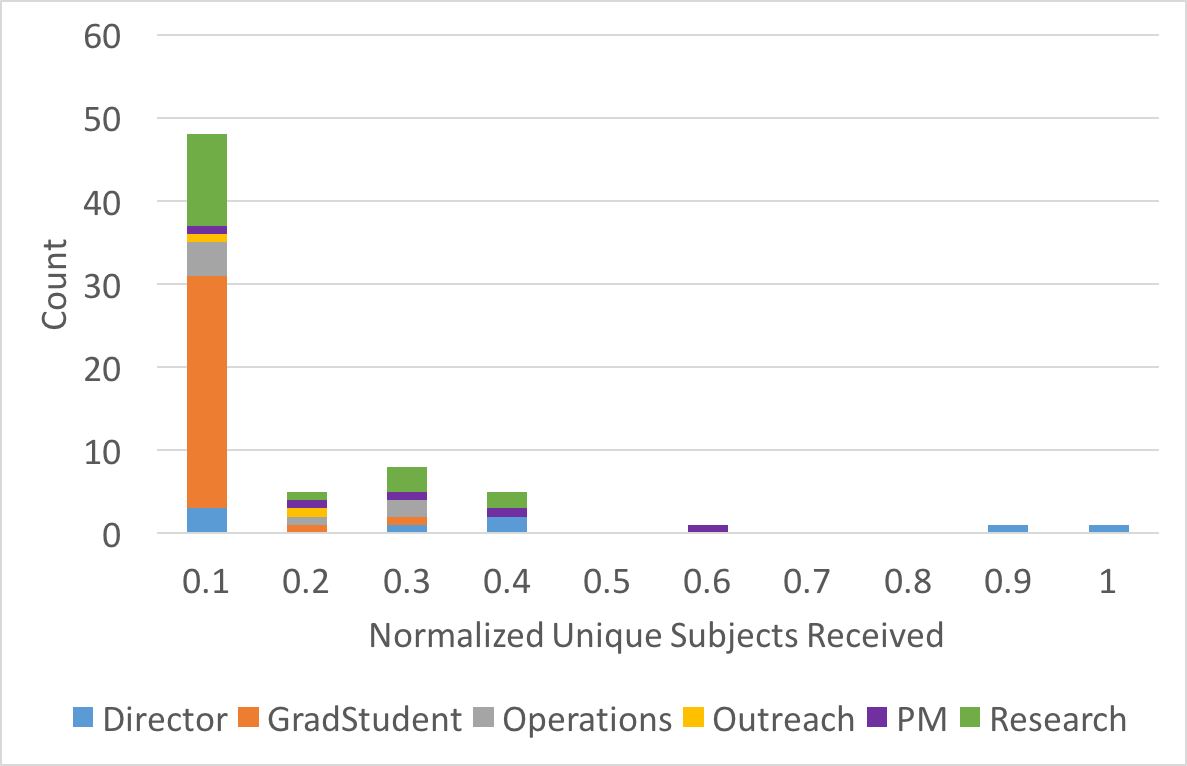
\includegraphics[width=0.4\textwidth]{Unique_subjects_rec_hist}
        \caption{Histogram of unique subjects received by job title.}
        \label{fig:traffic_ex_hist}
\end{figure}


\subsection{Social Network Features}
In addition to tracking metadata statistics, features can also be derived from modeling the emails as a social network.  A social network is composed of nodes, which represent people, and edges, which represent the emails between people.  For this analysis, two different graphs were generated.  In the full graph, an edge existed between any two individuals between which at least one email was exchanged.  A second graph was generated as a subset of the first.  In this partial graph, an edge was drawn between two nodes if they had exchanged at least 10 emails.  A representation of the full graph is shown below in Figure \ref{fig:adj_matrix}.  This figure is an adjacency matrix.  It has two axes, both representing the employees of the center.  The color at each coordinate indicates how much communication existed between the two employees.  Some employees never exchanged any emails, while others exchanged many.

\begin{figure}[H]
    \centering
        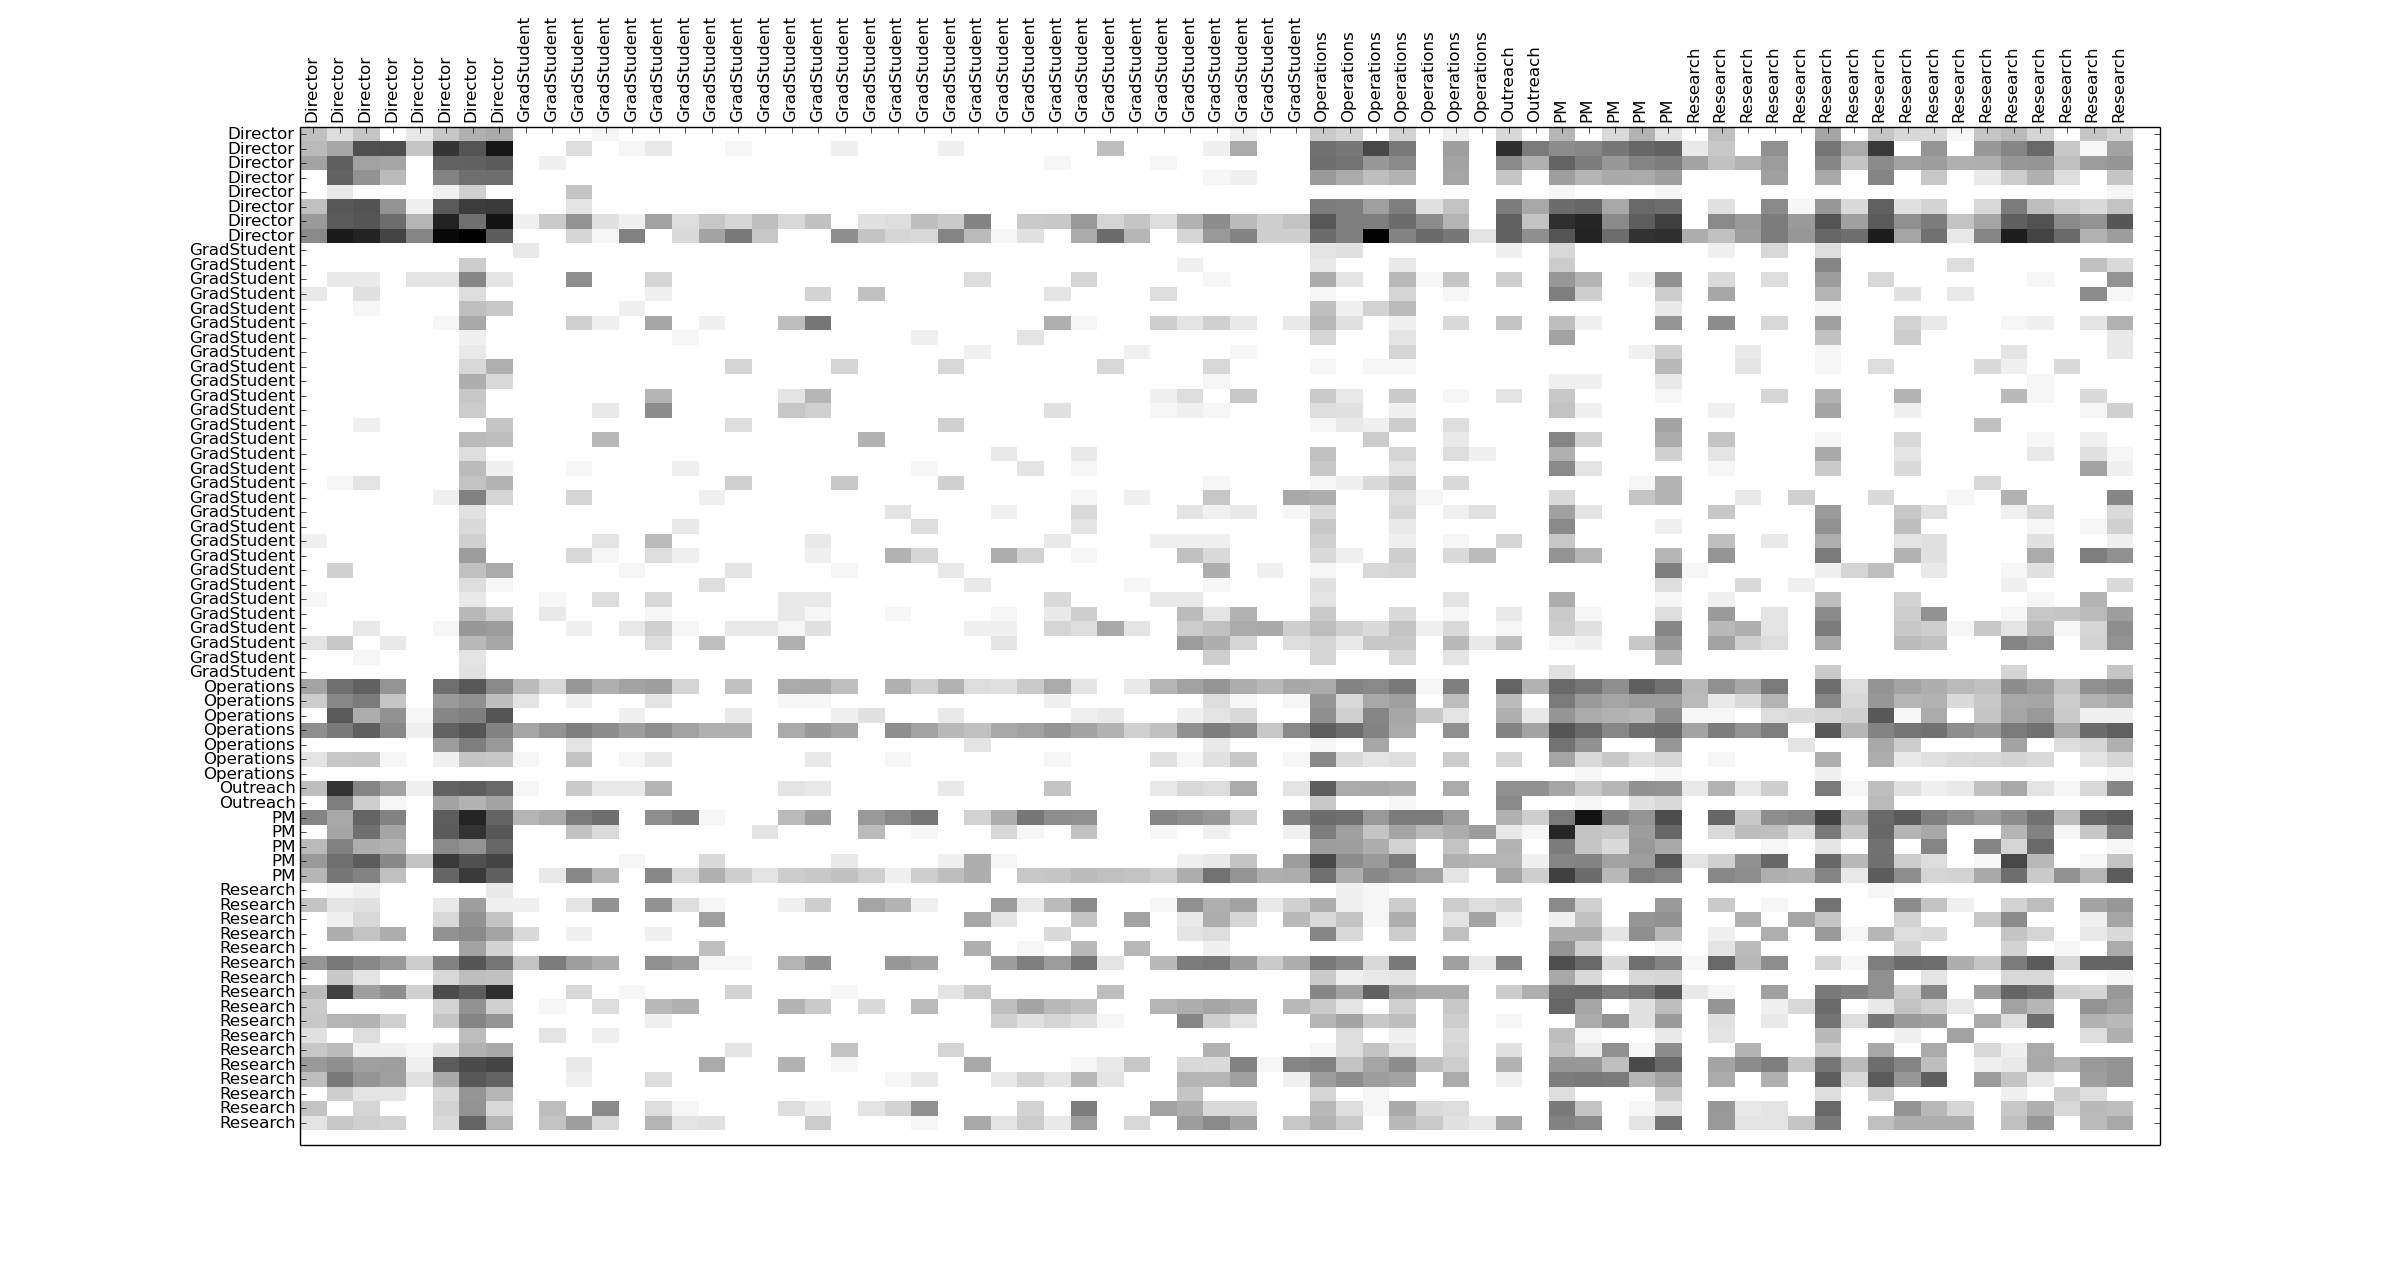
\includegraphics[width=0.5\textwidth]{adj_matrix}
        \caption{Adjacency matrix representing the social connections of the workplace.}
        \label{fig:adj_matrix}
\end{figure}

With this representation, several statistics can be calculated about the people in the graph.  The average neighbor degree was calculated for both the partial and the full graph.  The degree of a node $i$ is the number of other nodes connected to node $i$.  Therefore for a node $i$, this metric averages the degree of each node in the neighborhood of $i$, that is all nodes connected to $i$.  Mathematically, this is:
\begin{equation}
k_{avg,i} = \frac{1}{|N(i)|}\sum_{j \in N(i)}k_j
\end{equation}
where $N(i)$ are the neighbors of node $i$ and $k_j$ is the degree of node $j$.
The distances between nodes were also used to generate some features.  The average shortest path metric calculates the length of the shortest paths between node $i$ and all other nodes in the graph $G$, and it returns the average of these path lengths.  Similarly, the maximum shortest path length, or eccentricity, was used as a feature in the learning algorithm.  
\par
Many of the social features were based on existing graph theory concepts and algorithms. If a subgraph of a graph $G$ is maximally connected, that is all nodes are connected directly to each other, then this is called a clique.  The number of cliques to which a node belongs was used as a feature.  The hubs and authorities of each node in both graph were calculated.  The terms hubs and authorities come from the Hyperlink-Induced Topic Search (HITS algorithm) developed by \cite{kleinberg_hubs_1999}.  This algorithm was originally designed to rate web pages, but has since been applied to social networks. A node's authority is just that -- a measure of its importance over other nodes.  A node's hub score is a measure of how well-connected it is to other nodes.  The histogram of hub values in the full graph broken down by class is shown in Figure \ref{fig:social_ex_hist}.  Note that directors on average have the highest hub score and graduate students have the lowest. Another algorithm used to generate features was the pagerank algorithm, developed by Google \cite{page_pagerank_1999} also to rank webpages for search results.  The assumption is that the most important webpages will be linked to frequently by other pages.  Therefore, the ranking is determined by estimating the quality and quantity of links to a node.  The square clustering coefficient for each node was used as a feature.  This method, developed by \cite{lind_cycles_2005} measures the probability that two neighbors of node $i$ are also neighbors to a fourth node $j$.  The higher the clustering coefficient, the more connected the node is within its neighborhood.  The triangle clustering coefficient was also used as a metric.  This value, developed by \cite{saramaki_generalizations_2007}, is the same as the square clustering coefficient but instead determines the probability of connected triangles involving each node.

\begin{figure}[H]
    \centering
        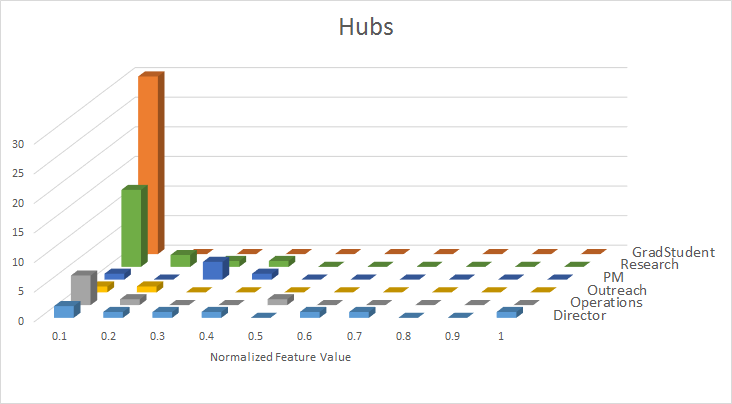
\includegraphics[width=0.4\textwidth]{Hubs_hist}
        \caption{Histogram of hubs from social graph by job title.}
        \label{fig:social_ex_hist}
\end{figure}

\par
By far, most of the social-based features came from different centrality measures.  This includes closeness centrality, betweenness centrality, degree centrality \cite{borgatti2011analyzing}, current flow closeness centrality, current flow betweenness centrality \cite{brandes2005centrality}, communicability centrality, communicability betweenness centrality \cite{estrada2008communicability}, and load centrality \cite{newman2001scientific}.
\par
All of these different graph statistics were used as inputs into the machine learning algorithm to characterize each node's importance in the social graph.


\section{Analysis} \label{Analysis}
The biggest limitation of this email dataset is the lack of participants.  Because of the low sample size, but great number of features, random forests were selected as the classification method.  The java-based software package Weka was used to run the random forest algorithm described in \cite{Breiman2001}.
\par
Random forests are an ensemble method of machine learning.  The random forest builds many random trees.  A random tree is a machine learning algorithm that uses training data learns a series of rules to use for classification.  These rules are constructed in a hierarchy that visually resembles a tree.  Each decision is based on what rule will maximize the information gained.  An example random tree with depth 3, meaning it has three levels of rules, is shown below in Figure \ref{fig:ex_tree}.
\begin{figure}[H]
    \centering
        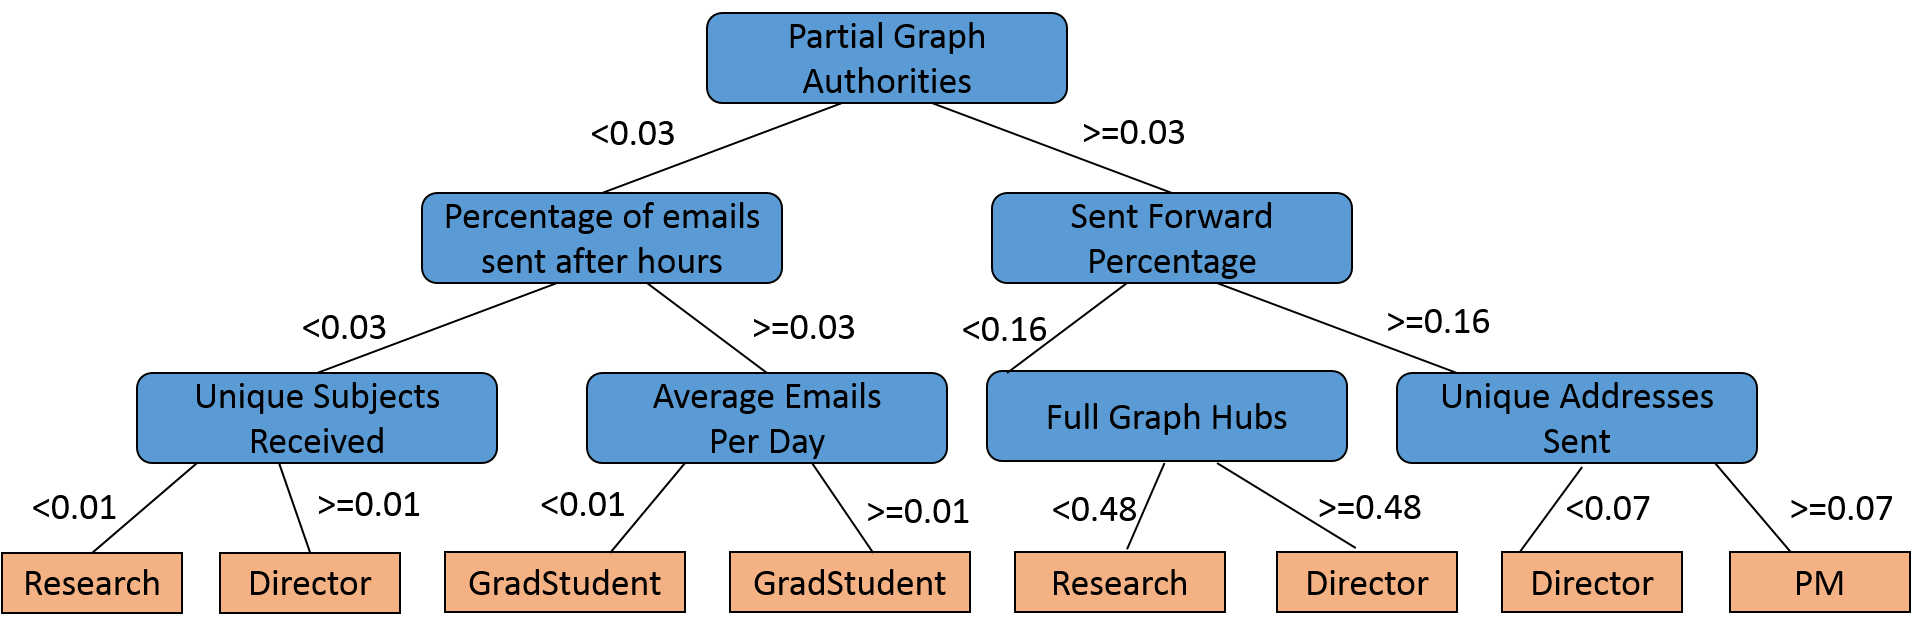
\includegraphics[width=0.5\textwidth]{3_level_tree}
        \caption{Example random tree of depth 3.}
        \label{fig:ex_tree}
\end{figure}
\par
Random forests build many, deep random trees with slight random variations.  Individually, these random trees will overfit the data.  However, these many random trees are combined through a process of bootstrap aggregating, or bagging.  This process involves each random tree generating a new training data set by sampling observations from the input training set with replacement.  These subsamples are used to build the random trees.  For this analysis, one third of the data was used as a test set and the rest was for training.  Just as the samples were subsampled, so were the features.  For each random tree, a subset of features is selected.  Only this subset can be used as rules for that tree.  In this implementation, each tree used a subsample of 15 features. Once a tree is built, the remaining samples from the training set are used as a test set and predicted labels for these points are generated. In this analysis, 750 random trees were generated. After all the trees are built, the majority vote on each sample prediction is the final predicted label.  Using this random forest model reduces the overall variance and increases the accuracy of the model compared to a single random tree.
\par
Random forests can be difficult to interpret because the ensemble method obscures which features are more meaningful than others.  To better understand which features were better label predictors, an attribute analysis algorithm was performed.  Since random trees use information gain to dictate splits, information gain was used as the evaluation criteria for the features.  Specifically, each attribute was evaluated by measured the information gain with respect to the class.  Information gain is calculated as follows for each attributed:
\begin{equation}
I(Class; Attribute) = H(Class) - H(Class | Attribute)
\end{equation} \label{eq:info_gained}
Where $I(Class; Attribute)$ represents the mutual information between the class and the attribute.  This value represents how much information, typically in terms of bits, knowledge of the attribute informs the prediction of the class.  In this model, both the attribute and the class are treated as random variables.  In the above equation $H(Class)$ is the entropy of the class variable.  The entropy of a random variable is a measure of the uncertainty associated with that random variable. In Equation \ref{eq:info_gained} above, $H(Class | Attribute)$ represents the conditional entropy of the Class given the Attribute value.  After this information gained value was calculated for each feature, they were ranked in order of most important to least.  Table \ref{tab:ranked_feats} shows the top twenty features from this analysis.


\begin{table}[H]
\centering
\caption{Top 20 features ranked by the information gain method.  Note that out of the to 20, there are 12 traffic-based features and 8 that are graph-based.}
\label{tab:ranked_feats}
\begin{tabular}{|l|l|l|}
\hline
Feature                                      & Feature      & InfoGained \\\hline
unique\_subjects\_received                   & Traffic      & 0.728  \\
total\_received\_signed                      & Traffic      & 0.728  \\
rec\_fw                                      & Traffic      & 0.719  \\
fg\_hubs                                     & Graph        & 0.589  \\
pg\_communicability\_centrality              & Graph        & 0.554  \\
pg\_communicability\_between\_cent           & Graph        & 0.554  \\
rec\_cc                                      & Traffic      & 0.507  \\
rec\_fw\_perc                                & Traffic      & 0.503  \\
pg\_degree\_centrality                       & Graph        & 0.492  \\
pg\_pagerank                                 & Graph        & 0.492  \\
pg\_current\_flow\_closeness\_cent           & Graph        & 0.492  \\
avg\_rec\_per\_day                           & Traffic      & 0.489  \\
avg\_emails\_per\_day                        & Traffic      & 0.479  \\
pg\_avg\_shortest\_paths                     & Graph        & 0.476  \\
pg\_closeness\_centrality                    & Graph        & 0.476  \\
unique\_addresses\_received\_signed          & Traffic      & 0.457  \\
sent\_cc                                     & Traffic      & 0.43   \\
rec\_re                                      & Traffic      & 0.43   \\
avg\_sent\_per\_day                          & Traffic      & 0.404  \\ \hline
\end{tabular}
\end{table}

The dataset did not have enough labeled employees to split the training and testing sets by people.  Instead, all emails in the database were randomly assigned to either the training or testing set.  Then, statistics were calculated for all 69 people using the training emails and testing emails separately.  This is a possible source of bias, but was the only choice for such a small sample size.  In order to determine the optimal percentage split for the emails, a series of runs was performed varying the size of the training data from 10\% to 90\% of the emails.  For each split, the data was run through the random forest algorithm and the prediction accuracy recorded.  The optimal test split was to use 50\% of the emails for training and the other 50\% for testing.  This result is plotted in Figure \ref{fig:split_analysis}.  Based on this result, I used a 50/50 split for the analysis of the classifier.

\begin{figure}[H]
    \centering
        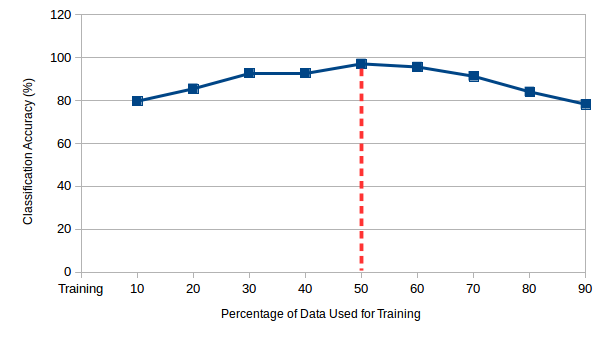
\includegraphics[width=0.4\textwidth]{SplitAnalysisWithLine}
        \caption{Prediction accuracy compared to percentage of data used for training.}
        \label{fig:split_analysis}
\end{figure}



\section{Results} \label{Results}
Two tests were run on the data.  In the first, the goal was to classify employees of the center based on their email behavior.  In the second, the official hierarchy from the organization chart was compared to relationships displayed in the data.

\subsection{Classification Results}
After splitting the data randomly in half, the training data was input into the random forest algorithm described in Section \ref{Analysis}.  The model from this algorithm was used to test the remaining data and output prediction labels.  These results are shown below in Figure \ref{fig:result_hist}.  The accuracy of this method using all features was 97.1\%.

\begin{figure}[H]
    \centering
        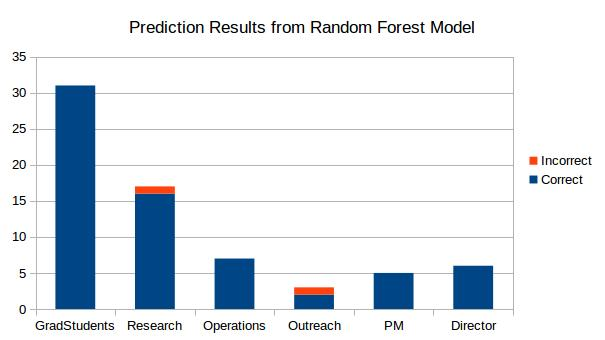
\includegraphics[width=0.5\textwidth]{Prediction_50_50_RF}
        \caption{Prediction accuracy for test set using Random Forest model.  Data was split such that 50\% was used as training data and 50\% was used as testing data.}
        \label{fig:result_hist}

\end{figure}
It is important to note that the two misclassifications above were for second ring employees.  All participants in the study were correctly classified, and 93.75\% of second ring employees were correctly classified.  The outreach employee operates as a teaching faculty for the center, and was classified as a graduate student, which makes sense.  There was the most training data available for graduate students, and only two training examples for outreach.  Similarly, the research employee was also mislabeled as a graduate student.  From our inside knowledge, we know that this person was a post-doctoral researcher.  Post-docs function similarly to both researchers and graduate students, so this classification also makes sense.
\par
Note that this method relies on some assumptions.  One is that employees with the same title exhibit similar email behavior.  Overall, based on the success of the algorithm and the distributions of the histograms, this seems to prove true.  Another premise underlying this analysis is that peoples' email behaviors are consistent over time.  This seems to be true as well.  However, it should be noted that results did vary slightly with different random splits.  Inconsistent behavior over time may have been a factor in this.

In order to determine which features were necessary to the analysis, the algorithm was run several times.  The first run used only the top 20 features from Figure \ref{tab:ranked_feats}, and the classification accuracy was recorded.  For each subsequent run, the least useful feature was removed from the input to the system.  Using only the top 20 features resulted in 3 classification errors, or 95.6\% accuracy.  This is only one more error than was found using all 101 features.  Even using just the top thee features resulted in classification accuracy over 80\%.  Therefore, a very good classifier can be built using much less features if the features are selected properly.
\begin{figure}[H]
    \centering
        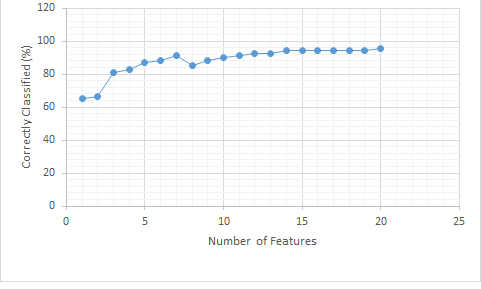
\includegraphics[width=0.4\textwidth]{FeatureAnalysis}
        \caption{Prediction accuracy compared to number of features used for analysis.}
        \label{fig:feat_analysis}
\end{figure}

\subsection{Hierarchy Analysis}
The ultimate goal of this research was to determine if the relationships present in the email data confirmed or conflicted with the official organization chart.  To test this, we compiled a list of the true directors for all non-director employees from the organization chart.  Next, we determined which director each of these employees emailed with the most.  Surprisingly, only 57.58\% of employees communicate most frequently with their official director.  This is understandable in cases where the director works in a different location than his or her employees.  This result points to possible issues in the construction of the organization chart.
\par
To further investigate the accuracy of the organization chart, we also compiled a list of the project manager for graduate students and researchers in the study.  In the case of an employee being on multiple projects, ground truth was selected to be the project that primarily funds the employee.  Some employees in this group were not included in this list because they did not have a project manager or because they worked at the center before an official project structure was in place.  This time, 72.73\% of graduate students and researchers communicate most frequently with their primary program manager.  The relation between employees to project managers appears to be stronger than that with directors.  Many of the discrepancies can be explained by employees participating in multiple projects and therefore having multiple project managers.


\section{Conclusions and Future Work} \label{Conclusions}
This work presented a new dataset, approximately the size of Enron, that was carefully collected from volunteers' emails with particular attention to protect participant privacy.  Unlike Enron, we used our inside knowledge, to label the people in this dataset has accurate job title.  A variety of statistics were calculated from this dataset, and from these statistics feature selection identified those key to making strong behavioral predictions.  Random Forests were shown to be powerful classifiers for this data.  They predicted employee job titles based on email data with very high accuracy, even employees that had only secondhand data was available.  Our intimate knoweldge is able to interpret the few classification errors produced by the algorithm.  However, there is the possibility of bias within this analysis in that training and testing are performed on the same people.  Therefore, in future work we hope to futher investigate this dataset and apply this wealth of information to other problems.  We also aim to evaluate these methods on other datasets, such as the Enron emails, and compare the features selected to identify any consistent predictors.


\clearpage
\Urlmuskip=0mu plus 1mu\relax
\bibliographystyle{named}
\bibliography{bib}


\end{document}